 \documentclass[UTF8,a4paper,12pt]{ctexbook} 

 \usepackage{graphicx}%学习插入图
 \usepackage{verbatim}%学习注释多行
 \usepackage{booktabs}%表格
 \usepackage{geometry}%图片
 \usepackage{amsmath}
 \usepackage{amssymb}
 \usepackage{listings}%代码
 \usepackage{xcolor}  %颜色
 \usepackage{enumitem}%列表格式
 \usepackage{tcolorbox}
 \usepackage{algorithm}  %format of the algorithm
 \usepackage{algorithmic}%format of the algorithm
 \usepackage{multirow}   %multirow for format of table
 \usepackage{tabularx} 	%表格排版格式控制
 \usepackage{array}	%表格排版格式控制
 \usepackage{hyperref} %超链接 \url{URL}
\usepackage{dirtree}
 \CTEXsetup[format+={\flushleft}]{section}

 %%%% 段落首行缩进两个字 %%%%
 \makeatletter
 \let\@afterindentfalse\@afterindenttrue
 \@afterindenttrue
 \makeatother
 \setlength{\parindent}{2em}  %中文缩进两个汉字位
 
 
 %%%% 下面的命令重定义页面边距,使其符合中文刊物习惯 %%%%
 \addtolength{\topmargin}{-54pt}
 \setlength{\oddsidemargin}{0.63cm}  % 3.17cm - 1 inch
 \setlength{\evensidemargin}{\oddsidemargin}
 \setlength{\textwidth}{14.66cm}
 \setlength{\textheight}{24.00cm}    % 24.62
 
 %%%% 下面的命令设置行间距与段落间距 %%%%
 \linespread{1.4}
 % \setlength{\parskip}{1ex}
 \setlength{\parskip}{0.5\baselineskip}
 
 %%%% 下面的命令定义图表、算法、公式 %%%%
 \newcommand{\EQ}[1]{$\textbf{EQ:}#1\ $}
 \newcommand{\ALGORITHM}[1]{$\textbf{Algorithm:}#1\ $}
 \newcommand{\Figure}[1]{$\textbf{Figure }#1\ $}
 
 %%%% 下面命令改变图表下标题的前缀 %%%%% 如:图-1、Fig-1
 \renewcommand{\figurename}{Fig}
 
 \geometry{left=1.6cm,right=1.8cm,top=2cm,bottom=1.7cm} %设置文章宽度
 %%%% 设置图片目录
 \graphicspath{{figure/}}
 
 \pagestyle{plain} 		  %设置页面布局

 %代码效果定义
 \definecolor{mygreen}{rgb}{0,0.6,0}
 \definecolor{mygray}{rgb}{0.5,0.5,0.5}
 \definecolor{mymauve}{rgb}{0.58,0,0.82}
 \lstset{ %
 	backgroundcolor=\color{white},   % choose the background color
 	basicstyle=\footnotesize\ttfamily,      % size of fonts used for the code
 	%stringstyle=\color{codepurple},
 	%basicstyle=\footnotesize,
 	%breakatwhitespace=false,         
 	%breaklines=true,                 
 	%captionpos=b,                    
 	%keepspaces=true,                 
 	%numbers=left,                    
 	%numbersep=5pt,                  
 	%showspaces=false,                
 	%showstringspaces=false,
 	%showtabs=false,        
 	columns=fullflexible,
 	breaklines=true,                 % automatic line breaking only at whitespace
 	captionpos=b,                    % sets the caption-position to bottom
 	tabsize=4,
 	commentstyle=\color{mygreen},    % comment style
 	escapeinside={\%*}{*)},          % if you want to add LaTeX within your code
 	keywordstyle=\color{blue},       % keyword style
 	stringstyle=\color{mymauve}\ttfamily,     % string literal style
 	frame=single,
 	rulesepcolor=\color{red!20!green!20!blue!20},
 	% identifierstyle=\color{red},
 	language=c++,
 }
 \author{\kaishu 郑华}
 \title{\heiti 图形学理论 笔记}
 
\begin{document}          %正文排版开始
 	\maketitle
 	\tableofcontents
 		
\chapter{背景知识}
	\section{绪论}
		计算机图形学是利用计算机研究图形的表示、生成、处理、显示的学科。
		
		\subsection{应用与意义}
			\begin{itemize}
				\item 电影 :科幻大片的特效
				\item 游戏 :图形地理、人物控制
				\item 计算机仿真
				\item CAD/CAM :设计、制造
	 			\item 建筑
				\item 可视化(科学):化学结构、生物
			\end{itemize}	
	
		\subsection{研究内容}
			\begin{itemize}
				\item 图形硬件、图形标准、图形交互技术
				\item 光栅图形生成算法
				\item 曲线曲面造型、实体造型
				\item 真实感图形绘制、科学计算可视化、计算机动画、自然景物仿真
				\item 虚拟现实
			\end{itemize}
			
	\section{涉及概念}
		\paragraph{图形与图象}
			\subparagraph{图像}
				计算机内以位图(Bitmap)形式存在的灰度信息。
		
			\subparagraph{图形}
				含有几何属性、更强调场景的几何表示,是由场景的几何模型和景物的物理属性共同组成的。
				
				图形主要分为两种:
				\begin{itemize}[itemindent = 1em]
					\item 基于线条信息表示
					\item 明暗图(\textbf{Shading})
				\end{itemize}
		
		\paragraph{图形学与CAD}
		\paragraph{图形学与模式识别}
		\paragraph{图形学与视觉}

	\section{历史}
		\begin{itemize}
			\item 细分曲面
			\item 光栅化图形:区域填充、裁剪、消隐等基本图形概念(70年代)
			\begin{enumerate}
				\item 光反射模型 70年(真实感图形学)
				\item 漫反射模型+插值 71年(明暗处理)
				\item 简单光照模型 75年(Phong 模型)
				\item 光投射模型 80年,并给出光线跟踪算法范例(Whitted 模型)
				\item 辐射度方法 84年
			\end{enumerate}

		\end{itemize}
		
	\section{杂志与会议}
		\paragraph{会议}
		\begin{itemize}
			\item Siggraph 
			\item Eurograph
			\item Pacific Graphics
			\item Computer Graphics International.
		\end{itemize}
		
		\paragraph{杂志}
			\begin{itemize}
				\item ACM Transaction on Graphics
				\item IEEE Computer Graphics and Application
				\item IEEE Visualization and Computer Graphics
			\end{itemize}


	\section{真实感绘制及重要概念}
		目的是模拟真实物体的物理属性,包括物体的形状,光学性质,表面的纹理和粗燥程度,以及物体间的相对位置,遮挡关系等。
		
		\dirtree{%
			.1 图形学理论.
			.2 \textbf{光照模型}.
			.3 简单光照模型.
			.3 局部光照模型.
			.3 整体光照模型.
			.2 \textbf{绘制方法}.
			.3 光线追踪.
			.3 辐射度.
			.2 \textbf{加速算法}.
			.3 包围盒树、自适应八叉树等.
			.3 阴影算法、纹理合成.
		}


\chapter{数学基础}
	参考:\url{https://blog.csdn.net/wangdingqiaoit/article/details/51383052}
	\section{向量}
		\subsection{点积}
	
		\subsection{差积}
		
	
	\section{矩阵}
		
	
	
	
	\section{GLM库}
	
	
	
	
	
\chapter{渲染管线}
	在给定虚拟相机、三维物体、光源、照明模式,以及纹理等诸多条件的情况下,生成或绘制出一幅2维图像的过程。
		\begin{figure}[H]
			\centering
			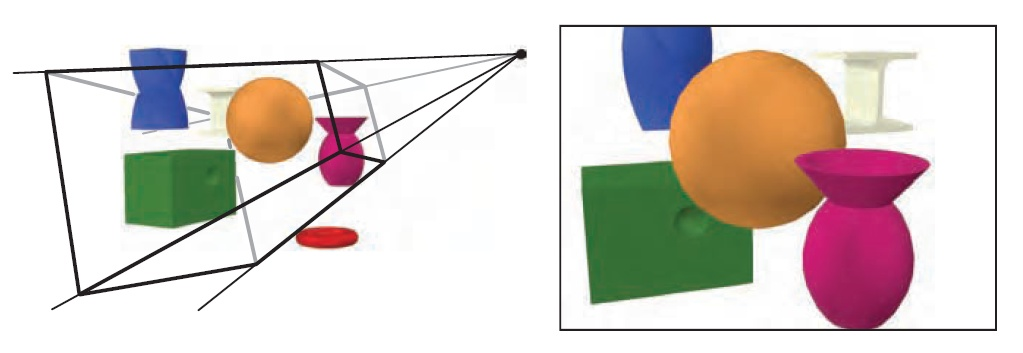
\includegraphics[scale=0.5]{Outline}
			\caption{渲染概述-三维到二维}
		\end{figure}
		
		而大体可以分为三部分:
		
		\begin{figure}[H]
			\centering
			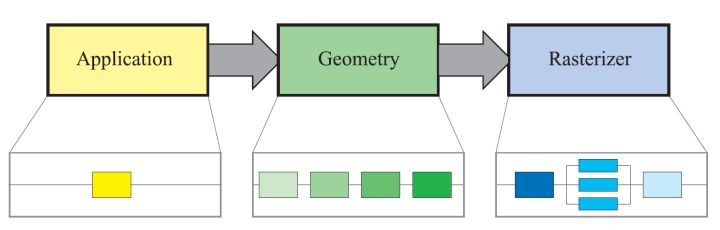
\includegraphics[scale=0.7]{Outline2}
			\caption{渲染结构}
		\end{figure}
		
	\section{应用阶段 - The Application Stage}
		应用程序阶段一般是图形渲染管线概念上的第一个阶段。应用程序阶段是通过软件方式来实现的阶段,开发者能够对该阶段发生的情况进行完全控制,可以通过改变实现方法来改变实际性能。其他阶段,他们全部或者部分建立在硬件基础上,因此要改变实现过程会非常困难。
		
		正因应用程序阶段是软件方式实现,因此不能像几何和光栅化阶段那样继续分为若干个子阶段。但为了提高性能,该阶段还是可以在几个并行处理器上同时执行。在CPU设计上,称这种形式为超标量体系(superscalar)结构,因为它可以在同一阶段同一时间做不同的几件事情。
		
		应用程序阶段通常实现的方法有\textbf{碰撞检测}、\textbf{加速算法}、\textbf{输入检测},\textbf{动画},\textbf{力反馈}以及\textbf{纹理动画},\textbf{变换仿真}、\textbf{几何变形},以及一些不在其他阶段执行的计算,如\textbf{层次视锥裁剪等加速算法}就可以在这里实现。
		
		应用程序阶段的主要任务:在应用程序阶段的末端,将需要在屏幕上(具体形式取决于具体输入设备)显示出来绘制的几何体(也就是绘制图元,rendering primitives,如点、线、矩形等)输入到绘制管线的下一个阶段。
		
		对于被渲染的每一帧,应用程序阶段将摄像机位置,光照和模型的图元输出到管线的下一个主要阶段——几何阶段。
		
	
	\section{几何阶段 - The Geometry Stage}
		负责大部分多边形操作和顶点操作。
			\begin{figure}[H]
				\centering
				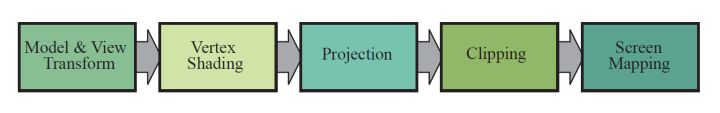
\includegraphics[scale=0.7]{Geometry}
				\caption{几何阶段演示}
			\end{figure}
		\subsection{模型视图变换阶段 - Model and View Transform} 
		
			模型变换的目的是将模型变换到适合渲染的空间当中,而视图变换的目的是\textbf{将摄像机位置放置于坐标原点},方便后续步骤的操作。
			
			在屏幕上的显示过程中,模型通常需要变换到若干不同的空间或坐标系中。模型变换的变换对象一般是模型的顶点和法线。物体的坐标称为模型坐标。世界空间是唯一的,所有的模型经过变换后都位于同一个空间中。
			
			不难理解,应该仅对相机(或者视点)可以看到的模型进行绘制。而相机在世界空间中有一个位置方向,用来放置和校准相机。
			
			为了便于投影和裁剪,必须对相机和所有的模型进行视点变换。变换的目的就是要把相机放在原点,然后进行视点校准,使其朝向Z轴负方向,y轴指向上方,x轴指向右边。在视点变换后,实际位置和方向就依赖于当前的API。我们称上述空间为\textbf{相机空间或者观察空间}。
		
				\begin{figure}[H]
					\centering
					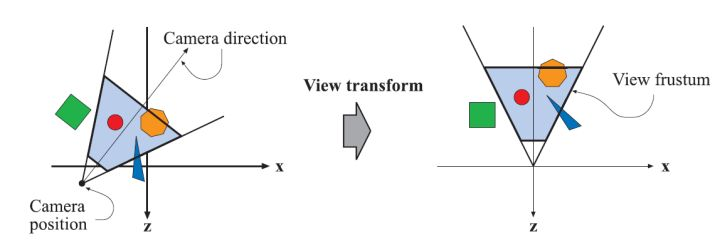
\includegraphics[scale=0.66]{ModelViewTransform}
					\caption{视图变换}
				\end{figure}
			
			在左图中,摄像机根据用户指定的位置进行放置和定位。在右图中,视点变换从原点沿着Z轴负方向对相机重新定位,这样可以使裁剪和投影操作更简单、更快速。可视范围是一个平截椎体,因此可以认为它是透视模式。	
			
			\subparagraph{总结}模型和视图变换阶段分为模型变换和视图变换。\textbf{模型变换}的目的是将模型变换到适合渲染的空间当中,而\textbf{视图变换}的目的是将摄像机放置于坐标原点,方便后续步骤的操作。
			
		\subsection{顶点着色阶段 - Vertex Shading} 
			顶点着色的目的在于\textbf{确定}模型上的\textbf{顶点处}材质的\textbf{光照效果}及\textbf{颜色}值。
			
			\color{blue}确定材质上的光照效果的这种操作被称为着色(shading),\color{black}着色过程涉及在对象上的各个点处计算\textbf{着色方程}(shading equation)。
			
			通常,这些计算中的一些在几何阶段期间在模型的顶点上执行(vertex shading),而其他计算可以在每像素光栅化(per-pixel rasterization)期间执行。\textbf{可以在每个顶点处存储各种材料数据},\textit{诸如点的位置,法线,颜色或计算着色方程所需的任何其它数字信息}。\color{red}\textbf{顶点着色的结果}(其可以是颜色,向量,纹理坐标或任何其他种类的阴着色数据)计算完成后,\textbf{会被发送到光栅化阶段以进行插值操作}。\color{black}
			
			通常,着色计算通常认为是在世界空间中进行的。在实践中,有时需要将相关实体(诸如相机和光源)转换到一些其它空间(诸如模型或观察空间)并在那里执行计算,也可以得到正确的结果。这是因为如果着色过程中所有的实体变换到了相同的空间,\textbf{着色计算中需要的诸如光源,相机和模型之间的相对关系是不会变的}。
			
		\subsection{投影阶段 - Projection} 
			就是将模型从三维空间投射到二维空间中的一个过程。
			
			在光照处理之后,渲染系统就开始进行投影操作,即将视体变换到一个对角顶点分别是(-1,-1,-1)和(1,1,1)单位立方体(unit cube)内,这个单位立方体通常也被称为规范立方体(Canonical View Volume,CVV)。
			目前,主要有两种投影方法,即:
			\begin{itemize}
				\item 正交投影:(orthographic projection,或称parallel projection)
				\item 透视投影:(perspective projection)。
			\end{itemize}
			
			\begin{figure}[H]
				\centering
				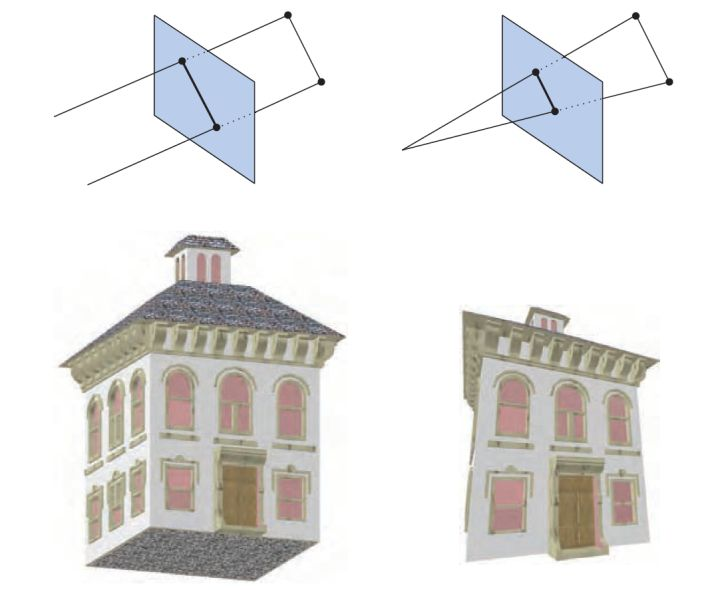
\includegraphics[scale=0.57]{project}
				\caption{投影演示}
			\end{figure}
			
			左边为正交投影,右边为透视投影。\textbf{正交投影}的可视体通常是一个矩形,正交投影可以把这个视体变换为单位立方体。正交投影的主要特性是平行线在变换之后彼此之间仍然保持平行,这种变换是平移与缩放的组合。\textbf{透视投影}比正交投影复杂一些。在这种投影中,越远离摄像机的物体,它在投影后看起来越小。更进一步来说,平行线将在地平线处会聚。透视投影的变换其实就是模拟人类感知物体的方式。
			
			正交投影和透视投影都可以通过4 x 4的矩阵来实现,在任何一种变换之后,都可以认为\textbf{模型位于归一化处理之后的设备坐标系中}。
			
			虽然这些矩阵变换是从一个可视体变换到另一个,但它们仍被称为投影,因为在完成显示后,\textbf{Z坐标将不会再保存于的得到的投影图片中}。通过这样的投影方法,\textbf{就将模型从三维空间投影到了二维的空间中}。
			
			\subparagraph{总结} 投影阶段就是将模型从三维空间投射到了二维的空间中的过程。
			
		\subsection{裁剪阶段 - Clipping} 
			就是对部分位于视体内部的图元进行裁剪操作。
			
			只有当图元完全或部分存在于视体(也就是上文的规范立方体,CVV)内部的时候,才需要将其发送到光栅化阶段,这个阶段可以把这些图元在屏幕上绘制出来。
			
			不难理解,一个图元相对视体内部的位置,分为三种情况:完全位于内部、完全位于外部、部分位于内部。所以就要分情况进行处理:
				\begin{itemize}
					\item 当图元完全位于视体内部,那么它可以直接进行下一个阶段。
					\item 当图元完全位于视体外部,不会进入下一个阶段,可直接丢弃,因为它们无需进行渲染。
					\item 当图元部分位于视体内部,则需要对那些部分位于视体内的图元进行裁剪处理。				
				\end{itemize}
			
			对部分位于视体内部的图元进行裁剪操作,这就是裁剪过程存在的意义。裁剪过程见下图。
				
				\begin{figure}[H]
					\centering
					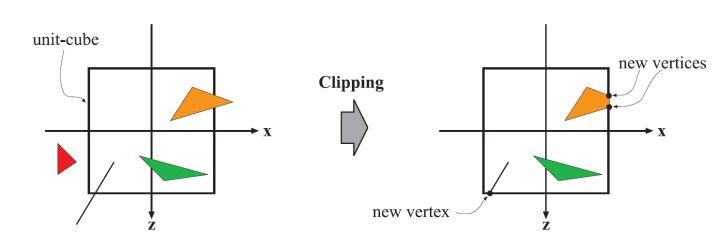
\includegraphics[scale=0.57]{clip}
					\caption{裁剪演示}
				\end{figure}
			
			投影变换后,\textbf{只对单位立方体内的图元}(\textit{相应的是视锥内可见图元})\textbf{继续进行处理},因此,\textbf{将单位立方体之外的图元剔除掉,保留单位立方体内部的图元},\textbf{同时沿着单位立方体将与单位立方体相交的图元裁剪掉},因此,就会产生新的图元,同时舍弃旧的图元。
			
		\subsection{屏幕映射阶段 - Screen Mapping} 
			就是将之前步骤得到的坐标映射到对应的屏幕坐标系上。
		
			只有在视体内部经过裁剪的图元,以及之前完全位于视体内部的图元,才可以进入到屏幕映射阶段。进入到这个阶段时,\textbf{坐标仍然是三维的}(\textbf{但显示状态在经过投影阶段后已经成了二维}),每个图元的x和y坐标变换到了屏幕坐标系中,屏幕坐标系连同z坐标一起称为窗口坐标系。
			
			假定在一个窗口里对场景进行绘制,窗口的最小坐标为(x1,y1),最大坐标为(x2,y2),其中x1<x2,y1<y2。屏幕映射首先进行平移,随后进行缩放,在映射过程中z坐标不受影响。新的x和y坐标称为屏幕坐标系,与z坐标一起(-1≦ z ≦ 1)进入光栅化阶段。如下图:
			
				\begin{figure}[H]
					\centering
					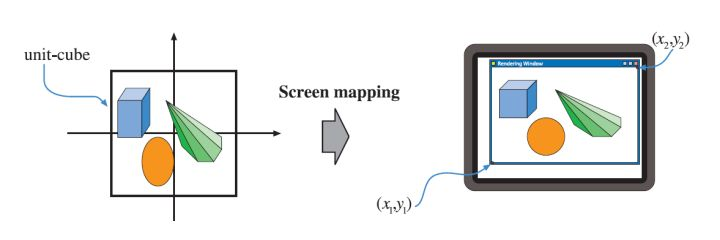
\includegraphics[scale=0.57]{scMap}
					\caption{屏幕映射演示}
				\end{figure}
	
			经过投影变换,图元全部位于单位立方体之内,而屏幕映射主要目的就是找到屏幕上对应的坐标
			
			屏幕映射阶段的一个常见困惑是整型和浮点型的点值如何与像素坐标(或纹理坐标)进行关联。可以使用Heckbert[书后参考文献第520篇]的策略,用一个转换公式进行解决。
			
			\subparagraph{总结}屏幕映射阶段的主要目的,就是将之前步骤得到的坐标映射到对应的屏幕坐标系上。
			
	\section{光栅化阶段 - The Rasterizer Stage}
		给定经过变换和投影之后的顶点,颜色以及纹理坐标,给每个像素正确配色,以便正确绘制整幅图像。
			\begin{figure}[H]
				\centering
				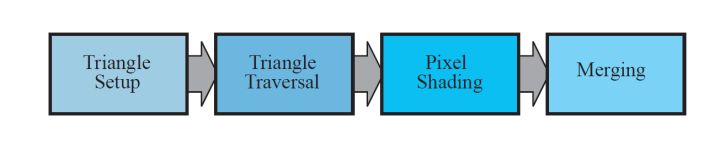
\includegraphics[scale=0.7]{Rasterization}
				\caption{光栅化演示}
			\end{figure}
			
			\subsection{三角形设定阶段 - Triangle Setup}
				三角形设定阶段主要用来计算三角形表面的差异和三角形表面的其他相关数据。
				
				该数据主要用于扫描转换(scan conversion),以及由几何阶段处理的各种着色数据的插值操作所用。 该过程在专门为其设计的硬件上执行。
				 
			\subsection{三角形遍历阶段 - Triangle Traversal}
				在三角形遍历阶段将进行\textbf{逐像素检查操作},\textbf{检查该像素处的像素中心是否由三角形覆盖},\textbf{而对于有三角形部分重合的像素,将在其重合部分生成片段(fragment)}。
				
				找到哪些采样点或像素在三角形中的过程通常叫三角形遍历(TriangleTraversal)或扫描转换(scan conversion)。\textbf{每个三角形片段的属性均由三个三角形顶点的数据插值而生成}。这些属性包括片段的深度,以及来自几何阶段的着色数据。

			\subsection{像素着色阶段 - Pixel Shading}
				所有逐像素的着色计算都在像素着色阶段进行,使用插值得来的着色数据作为输入,输出结果为一种或多种将被传送到下一阶段的颜色信息。纹理贴图操作就是在这阶段进行的。
				
				像素着色阶段是在可编程GPU内执行的,在这一阶段有大量的技术可以使用,其中最常见,最重要的技术之一就是纹理贴图(Texturing)。纹理贴图在书的第六章会详细讲到。简单来说,纹理贴图就是将指定图片“贴”到指定物体上的过程。而指定的图片可以是一维,二维,或者三维的,其中,自然是二维图片最为常见。如下图所示:
					\begin{figure}[H]
						\centering
						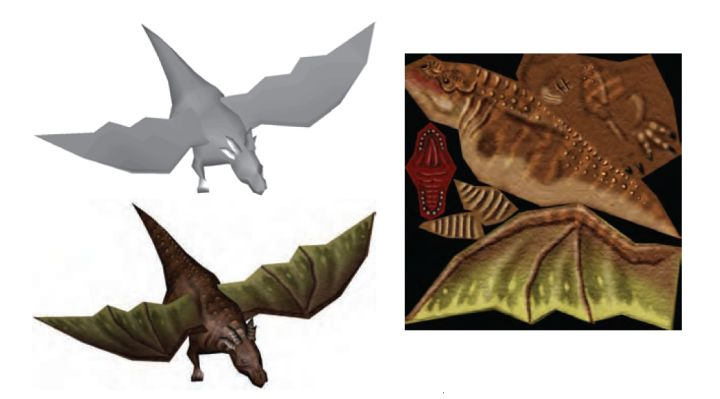
\includegraphics[scale=0.57]{PixShader}
						\caption{片段着色器演示}
					\end{figure}
				
				左上角为一没有纹理贴图的飞龙模型。左下角为一贴上图像纹理的飞龙。右图为所用的纹理贴图。
				
			\subsection{融合 - Merging}
				每个像素的信息都储存在\textbf{颜色缓冲器}中,而颜色缓冲器是一个颜色的矩阵列(每种颜色包含红、绿、蓝三个分量)。融合阶段的主要任务是合成当前储存于缓冲器中的由之前的像素着色阶段产生的片段颜色。不像其它着色阶段,通常运行该阶段的GPU子单元并非完全可编程的,但其高度可配置,可支持多种特效。
				
				此外,这个阶段还负责可见性问题的处理。这意味着当绘制完整场景的时候,颜色缓冲器中应该还包含从相机视点处可以观察到的场景图元。对于大多数图形硬件来说,这个过程是通过Z缓冲(也称\textbf{深度缓冲器})算法来实现的。Z缓冲算法非常简单,具有O(n)复杂度(n是需要绘制的像素数量),只要对每个图元计算出相应的像素z值,就可以使用这种方法,大概内容是:
				
				\textbf{Z缓冲器器}和颜色缓冲器形状大小一样,每个像素都存储着一个z值,这个z值是从相机到最近图元之间的距离。每次将一个图元绘制为相应像素时,需要计算像素位置处图元的z值,并与同一像素处的z缓冲器内容进行比较。如果新计算出的z值,远远小于z缓冲器中的z值,那么说明即将绘制的图元与相机的距离比原来距离相机最近的图元还要近。这样,像素的z值和颜色就由当前图元对应的值和颜色进行更新。反之,若计算出的z值远远大于z缓冲器中的z值,那么z缓冲器和颜色缓冲器中的值就无需改变。
														
				上面刚说到,颜色缓冲器用来存储颜色,z缓冲器用来存储每个像素的z值,还有其他缓冲器可以用来过滤和捕获片段信息。
				
				\begin{itemize}	
					\item 比如\textbf{alpha通道}(alpha channel)和\textbf{颜色缓冲器}\textit{联系在一起}可以存储一个与每个像素相关的不透明值。可选的alpha测试可在深度测试执行前在传入片段上运行。片段的alpha值与参考值作某些特定的测试(如等于,大于等),如果片断未能通过测试,它将不再进行进一步的处理。alpha测试经常用于不影响深度缓存的全透明片段(见6.6节)的处理。
									
					\item \textbf{模板缓冲器}(stencil buffer)是用于记录所呈现图元位置的离屏缓存。每个像素通常与占用8个位。图元可使用各种方法渲染到模板缓冲器中,而缓冲器中的内容可以控制颜色缓存和Z缓存的渲染。举个例子,假设在模版缓冲器中绘制出了一个实心圆形,那么可以使用一系列操作符来将后续的图元仅在圆形所出现的像素处绘制,类似一个mask的操作。模板缓冲器是制作特效的强大工具。而在管线末端的所有这些功能都叫做光栅操作(raster operations ,ROP)或混合操作(blend operations)。
									
					\item \textbf{帧缓冲器}(frame buffer)通常包含一个系统所具有的所有缓冲器,但有时也可以认为是颜色缓冲器和z缓冲器的组合。
									
					\item \textbf{累计缓冲器}(accumulation buffer),是1990年,Haeberli和Akeley提出的一种缓冲器,是对帧缓冲器的补充。这个缓冲器可以用一组操作符对图像进行累积。例如,为了产生运动模糊(motion blur.,可以对一系列物体运动的图像进行累积和平均。此外,其他的一些可产生的效果包括景深(e depth of field),反走样(antialiasing)和软阴影(soft shadows)等。
				\end{itemize}

				而当图元通过光栅化阶段之后,从相机视点处看到的东西就可以在荧幕上显示出来。为了避免观察者体验到对图元进行处理并发送到屏幕的过程,图形系统一般使用了双缓冲(double buffering)机制,这意味着屏幕绘制是在一个后置缓冲器(backbuffer)中以离屏的方式进行的。一旦屏幕已在后置缓冲器中绘制,后置缓冲器中的内容就不断与已经在屏幕上显示过的前置缓冲器中的内容进行交换。注意,只有当不影响显示的时候,才进行交换。
				
				\subparagraph{总结}融合阶段的主要任务是合成当前储存于缓冲器中的由之前的像素着色阶段产生的片段颜色。此外,融合阶段还负责可见性问题(Z缓冲相关)的处理。

	\section{可编程部分演示}
		\begin{figure}[H]
			\centering
			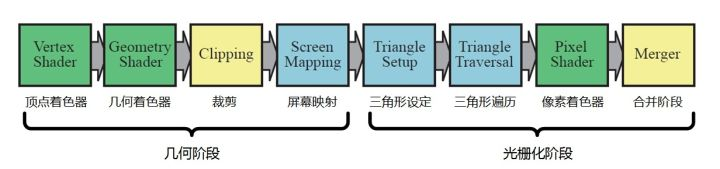
\includegraphics[scale=0.57]{ProgramAble}
			\caption{可编程阶段演示}
		\end{figure}	
		
		其中,\color{olive}绿色的阶段表示完全可编程的。\color{yellow}黄色表示可配置,但不可编程。\color{blue}蓝色的阶段完全固定。\color{black}
		
	\section{三大测试}
		参考U3D Shader -> Shader 着色器一章。
		
		\url{https://blog.csdn.net/wangdingqiaoit/article/category/2107037}
	
	\section{混合}
	
	
	\section{背面剔除}
	
	
	\section{渲染队列}
		\url{https://blog.csdn.net/puppet_master/article/details/53900568}
		

\chapter{线性代数 Linear}
	\section{向量}
	
	\section{矩阵}


		
\chapter{变换 Transform}
	见OpenGL\_4.5笔记


\chapter{视觉外观}
	\section{光照与材质}
		\subsection{光照现象-散射与吸收}
		
		\subsection{表面粗糙度}
		

	\section{着色原理}
		\subsection{着色与着色方程}
		
		\subsection{三种着色处理方法}
		
		
	\section{抗锯齿与常见抗锯齿类型}
		抗锯齿(英语:Anti-Aliasing,简称AA),也译为边缘柔化、消除混叠、抗图像折叠有损,反走样等。它是一种消除显示器输出的画面中图物边缘出现凹凸锯齿的技术,那些凹凸的锯齿通常因为高分辨率的信号以低分辨率表示或无法准确运算出3D图形坐标定位时所导致的图形混叠(aliasing)而产生的,抗锯齿技术能有效地解决这些问题。
		
		下面将常见的几种抗锯齿类型进行总结介绍,也包括RTR3中没有讲到的,最近几年新提出的常见抗锯齿类型。
		
		\subsection{超级采样抗锯齿(SSAA)}
		
		\subsection{多重采样抗锯齿(MSAA)}
		
		\subsection{覆盖采样抗锯齿(CSAA)}
		
		\subsection{高分辨率抗锯齿(HRAA)}
		
		\subsection{可编程过滤抗锯齿(CFAA)}
		
		\subsection{形态抗锯齿(MLAA)}
		
		\subsection{快速近似抗锯齿(FXAA)}
		
		\subsection{时间性抗锯齿(TXAA)}
		
		\subsection{多帧采样抗锯齿(MFAA)}
		
	\section{透明渲染与透明排序}
		\subsection{透明渲染}
		
		\subsection{透明排序}
			\paragraph{深度缓存(Z-Buffer)}
			
			\paragraph{画家算法(Painter's Algorithm)}
			
			\paragraph{加权平均值算法(Weighted Average)}
			
			\paragraph{深度剥离算法(Depth Peeling)}

	\section{伽马矫正}
	
	\section{参考文献}
			参考于:\url{https://zhuanlan.zhihu.com/p/27234482}
	

	
			
\chapter{纹理贴图}
	\section{纹理管线}
		纹理(Texturing)是一种针对物体表面属性进行“建模”的高效技术。图像纹理中的像素通常被称为纹素(Texels),区别于屏幕上的像素。根据Kershaw的术语,\textit{通过将投影方程(projector function)运用于空间中的点 ,从而得到一组称为参数空间值(parameter-spacevalues)的关于纹理的数值}。这个过程就称为贴图(Mapping,也称映射 ),也就是\textbf{纹理贴图}(Texture Mapping,也称纹理映射 )这个词的由来。
		
		纹理贴图可以用一个通用的纹理管线来进行描述。纹理贴图过程的\textbf{初始点}是空间中的一个位置。这个位置\textbf{可以基于世界空间},但是\textbf{更常见的是基于模型空间}。因为若此位置是基于模型空间的,当模型移动时,其纹理才会随之移动。
		
		如下图为一个纹理管线(The Texturing Pipeline),也就是单个纹理应用纹理贴图的详细过程,而此管线有点复杂的原因是每一步均为用户提供了有效的控制。
			\begin{figure}[H]
				\centering
				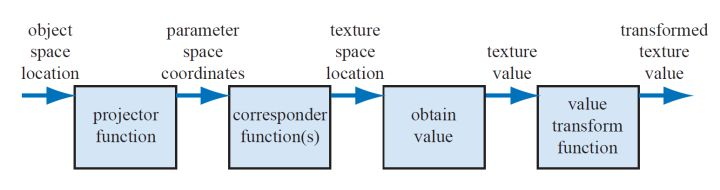
\includegraphics[scale=0.67]{TexturePipeline}
				\caption{单个纹理的通用纹理管线}
			\end{figure}
			
		下面是对上图中描述的纹理管线的分步概述:
			\begin{enumerate}[itemindent = 2em]
				\item 通过将投影方程(projector function)运用于空间中的点 ,从而得到一组称为参数空间值(parameter-space values)的\textbf{关于纹理的数值}。
				\item 在使用这些新值访问纹理之前,可以使用一个或者多个映射函数(corresponder function)将\textbf{参数空间值}(parameter-space values )转换到\textbf{纹理空间}。
				\item 使用这些纹理空间值(texture-space locations)\textbf{从纹理中获取相应的值}(obtain value)。例如,可以使用图像纹理的数组索引来检索像素值。
				\item 再使用值变换函数(value transform function)对检索结果进行值变换,最后使用得到的新值来改变表面属性,如材质或者着色法线等等。
			\end{enumerate}

		而如下这个例子应该对理解纹理管线有所帮助。下例将描述出使用纹理管线,一个多边形在给定一张砖块纹理时在其表面上生成样本时(如下图)发生了哪些过程。
			\begin{figure}[H]
				\centering
				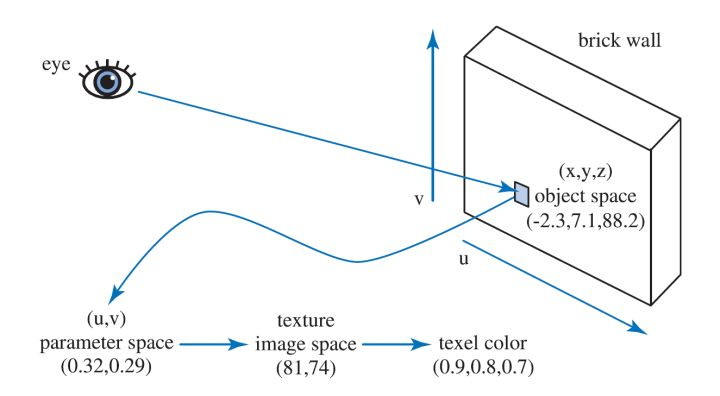
\includegraphics[scale=0.67]{TexturePipeline2}
				\caption{一个砖墙的纹理管线过程}
			\end{figure}
		
		在具体的参考帧画面中找到\textbf{物体空间中的位置(x,y,z)},如图中点(-2.3,7.1,88.2),然后\textbf{对该位置运用投影函数}。\color{blue}\textbf{这个投影函数通常将向量(x,y,z)转换为一个二元向量(u,v)}\color{black}。在此示例中使用的投影函数是一个正交投影,类似一个投影仪,将具有光泽的砖墙图像投影到多边形表面上。再考虑砖墙这边,其实这个投影过程就是将砖墙平面上的点变换为值域为0到1之间的一对(u,v)值,如图,(0.32,0.29)就是这个我们通过投影函数得到的uv值。\textbf{而我们图像(纹理)的分辨率是256 x 256,所以,将256分别乘以(0.32,0.29),去掉小数点,得到纹理坐标(81, 74)。}通过这个纹理坐标,可以\textbf{在纹理贴图上查找到坐标对应的颜色值},所以,我们接着找到砖块图像上像素位置为(81,74)处的点,得到颜色(0.9,0.8,0.7)。而由于原始砖墙的颜色太暗,因此可以使用一个值变换函数,给每个向量乘以1.1,就可以得到我们纹理管线过程的结果——颜色值(0.99,0.88,0.77)。
		
		随后,我们就可以将此值用于着色方程,作为物体的漫反射颜色值,替换掉之前的漫反射颜色。
		
		下面是纹理管线中主要的两个组成,投影函数(The Projector Function)和映射函数(The Corresponder Function)。
			
	\section{投影函数}
		作为\textbf{纹理管线的第一步},投影函数的功能就是\textbf{将空间中的三维点转化为纹理坐标},也就是\textbf{获取表面的位置并将其投影到参数空间中}。
		
		在常规情况下,投影函数通常在美术建模阶段使用,并将投影结果存储于顶点数据中。也就是说,在软件开发过程中,我们一般不会去用投影函数去计算得到投影结果,\textbf{而是直接使用在美术建模过程中,已经存储在模型顶点数据中的投影结果}。
		
	\section{映射函数}
		映射函数(The Corresponder Function)的作用是将参数空间坐标(parameter-space coordinates)转换为纹理空间位置(texture space locations)。
		
		我们知道图像会出现在物体表面的(u,v)位置上,且uv值的正常范围在[0,1)范围内。超出这个值域的纹理,其显示方式便可以由映射函数(The Corresponder Function)来决定。
		
		在OpenGL中,这类映射函数称为“封装模式(Warapping Mode)”,在Direct3D中,这类函数叫做“寻址模式(Texture Addressing Mode)”。最常见的映射函数有以下几种:
			
			\begin{figure}[H]
				\centering
				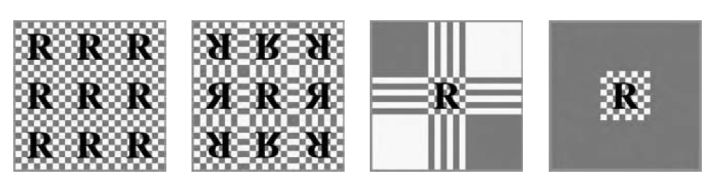
\includegraphics[scale=0.57]{Mapping}
				\caption{映射方式}
			\end{figure}
			
			\begin{itemize}
				\item \textbf{重复寻址模式},\verb|wrap| (DirectX), \verb|repeat| (OpenGL)。图像在表面上重复出现。
				\item \textbf{镜像寻址模式},\verb|mirror|。图像在物体表面上不断重复,但每次重复时对图像进行镜像或者反转。
				\item \textbf{夹取寻址模式},\verb|clamp| (DirectX) ,clamp to edge (OpenGL)。夹取纹理寻址模式将纹理坐标夹取在[0.0,1.0]之间,也就是说,在[0.0,1.0]之间就是把纹理复制一遍,然后对于[0.0,1.0]之外的内容,将边缘的内容沿着u轴和v轴进行延伸。
				\item \textbf{边框颜色寻址模式},\verb|border| (DirectX) ,clamp to border (OpenGL)。边框颜色寻址模式就是在[0.0,1.0]之间绘制纹理,然后[0.0,1.0]之外的内容就用边框颜色填充。		
			\end{itemize}

		另外,每个纹理轴可以使用不同的映射函数。例如在u轴使用重复寻址模式,在v轴使用夹取寻址模式。
		
	\section{体纹理}
	
	\section{立方体贴图}
		立方体纹理(cube texture)或立方体贴图(cube map)是一种特殊的纹理技术,它用6幅二维纹理图像构成一个以原点为中心的纹理立方体,这每个2D纹理是一个立方体(cube)的一个面。对于每个片段,纹理坐标(s, t, r)被当作方向向量看待,每个纹素(texel)都表示从原点所看到的纹理立方体上的图像。
		
			\begin{figure}[H]
				\centering
				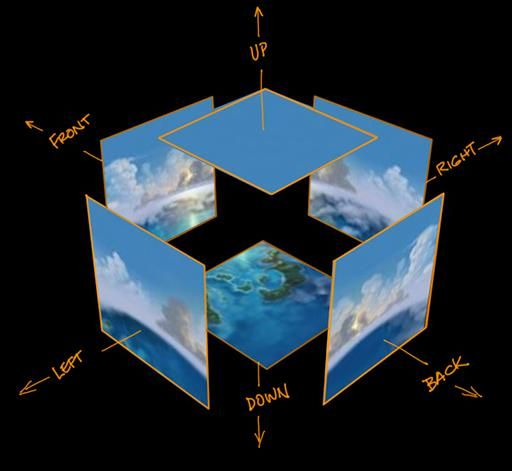
\includegraphics[scale=0.57]{cubeMap}
				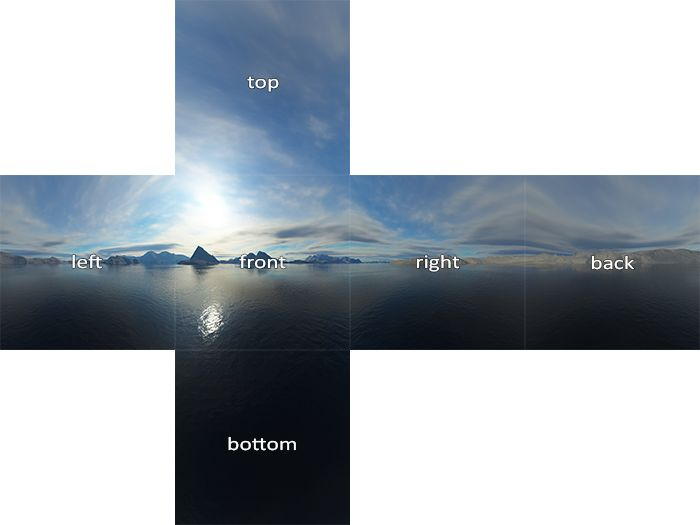
\includegraphics[scale=0.57]{cubeMap1}
				\caption{立方体贴图}
			\end{figure}
		
		可以使用三分量纹理坐标向量来访问立方体贴图中的数据,该矢量指定了从立方体中心向外指向的光线的方向。选择具有最大绝对值的纹理坐标对应的相应的面。(例如:对于给定的矢量(−3.2, 5.1, −8.4),就选择-Z面),而对剩下的两个坐标除以最大绝对值坐标的绝对值,即8.4。 那么就将剩下的两个坐标的范围转换到了-1到1,然后重映射到[0,1]范围,以方便纹理坐标的计算。例如,坐标(-3.2,5.1)映射到((-3.2 / 8.4 + 1)/ 2,(5.1/ 8.4 + 1)/ 2)≈(0.31,0.80)。
		
		立方体贴图支持\textbf{双线性滤波}以及\textbf{mip mapping},但问题可以可能会在贴图接缝处出现。有一些处理立方体贴图专业的工具在滤波时考虑到了可能的各种因素,如ATI公司的CubeMapGen,采用来自其他面的相邻样本创建\textbf{mipmap链},并考虑每个纹素的角度范围,可以得到比较不错的效果。
				
	\section{纹理缓存}
	
	\section{纹理压缩}
	
	\section{程序贴图纹理}
	
	\section{凹凸贴图}
		凹凸贴图(Bump Mapping)思想最早是由图形学届大牛中的大牛Jim Blinn提出,后来的Normal Mapping,Parallax Mapping,Parallax Occulision Mapping,Relief Mapping等等,均是基于同样的思想,只是考虑得越来越全面,效果也越来越逼真。
		
		\begin{figure}[H]
			\centering
			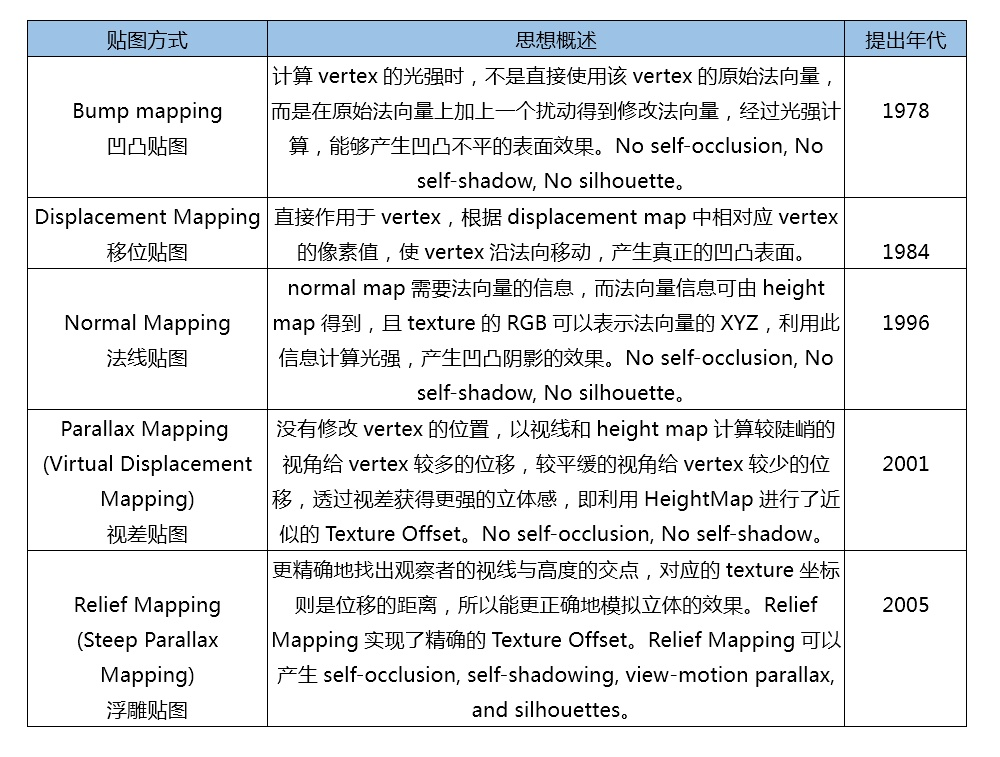
\includegraphics[scale=0.53]{normMap}
			\caption{凹凸贴图对比}
		\end{figure}
		
		除了Displacement Mapping方法以外,其他的几种改进一般都是通过修改每像素着色方程来实现,关键思想是访问纹理来修改表面的法线,而不是改变光照方程中的颜色分量。物体表面的几何法线保持不变,我们修改的只是照明方程中使用的法线值。他们比单独的纹理有更好的三维感官,但是显然还是比不上实际的三维几何体。
		
		\subsection{移位贴图}
		
		\subsection{法线贴图}
			\paragraph{高度图或灰度图}
				一张二维纹理有两个维度 $u$ 和 $v$,但其实,高度($h$)可以算第三个维度。有了高度,一张二维纹理就可以想象成一个三维的物体了。
					\begin{figure}[H]
						\centering
						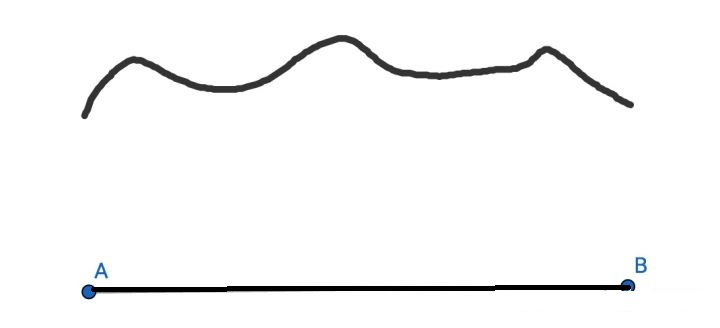
\includegraphics[scale=0.54]{norMap}
						\caption{UV例子}
					\end{figure}
				
				先来考虑只有 $u$ 方向的情况,如图所示, $A$ 和 $B$ 是纹理中的两个点, $uv$ 坐标分别是 (0, 0) 和 (1, 0),上方黑线表示点对应的高度,那么显然,只要求出 $u$ 方向上的高度函数在某一点的切线,就能求出垂直于他的法线了。同理, $v$ 方向也是如此。也就是说,如果有纹理的高度信息,那么就能计算出纹理中每一个像素的法线了。
				
				所以计算法线需要一张高度图,它表示纹理中每一个点对应的高度。
				
				但其实并不需要求出每个纹理像素上 $uv$ 方向各自的法线,只需要求出 $uv$ 方向上高度函数的切线,再做一个叉积,即可计算出对应的法线了。
				
				如果没有高度图,也可以用灰度图代替,灰度图就是把 $rgb$ 三个颜色分量做一个加权平均,有很多种算法提取灰度值,这里用一个比较常用的基于人眼感知的灰度值提取公式。
				
				$$color.r * 0.2126 + color.g * 0.7152 + color.b * 0.0722$$
				
				这个公式是由人眼对不同颜色敏感度不同得来的,这里无需过多计较,直接把提取出来的灰度值作为高度值即可。
			\paragraph{计算方法}
			
			\paragraph{实例}
			
		\subsection{视差贴图}
		
		\subsection{浮雕贴图}
	
	\section{参考}
		参考于:\url{https://zhuanlan.zhihu.com/p/27551369}
		
		法线贴图:\url{https://www.zhihu.com/people/zheng-hua-31-46/following}
		
		
\chapter{光照}


\chapter{基于图像的效果}



\chapter{参考学习路线}					
	
	\section{OS 基础}
		《Programming Windows 5th》只需要看前面几章,理解 Win32 消息循环即可。
	
		《Multithreading Applications in Win32》,理解多线程是怎么回事;
	
	\section{GUI}
	 	WPF、MFC
	
	\section{3D 图形学}
		二选一,我推荐 handmadehero,因为有很详细的视频教程。
		
		\url{https://handmadehero.org/}
		
		\url{http://frustum.org/3d/}从最开始的 demo 开始,用 DX 全部写一遍。
	
	\section{基础篇}
		\begin{itemize}
			\item 上篇,各种概念与技术。《Fundamentals of Computer Graphics 3rd》 or 《Computer Graphics - Principles and Practice》
			\item 中篇,各种算法。《Real-Time Rendering 4th》
			\item 下篇,高阶追求。《Physically Based Rendering - From Theory To Implementation 2nd》
			\item 杂篇1,只谈数学,《3D Math Primer for Graphics and Game Development 2nd》
			\item 杂篇2,同上,《Mathematics for 3D Game Programming and Computer Graphics 3rd》
		\end{itemize}
		
	\section{API 之术(DX9/11 or OpenGL)}
		\begin{itemize}
			\item 《3D绘图程序设计》,dx9/10/ogl 实现各种3D游戏需要的效果
			\item 《More OpenGL Game Programming》,如何用 gl 实现各种中高级效果
			\item 《Introduction to 3D Game Programming with DirectX 9.0c - A Shader Approach》,龙书
			\item 《Introduction to 3D Game Programming with DirectX 11》,龙书 DX11 版
			\item 《Practical Rendering and Computation with Direct3D 11》,DX11 宝典
			\item 《OpenGL Programming Guide》,OpenGL 宝典		
			\item 《OpenGL Shading Language》,glsl 宝典			
		\end{itemize}
	
	\section{引擎设计}		
		David Eberly 的《3D Game Engine Design》,WildMagic,这有一个完整的引擎实现
		
		Jason Gregory 的《Game Engine Architecture》
		
		《Character Animation with Direct3D》,专注讲 model、animation 的。
		
	\section{各种技巧}
		ShaderX 系列
		《Real Time Collision Detection》
		《Real Time Cameras》
		《Real-Time Shadows》

	  
\end{document} 
 		    